
\newif\ifshowsolutions
\showsolutionstrue
\documentclass{article}
\usepackage{listings}
\usepackage{amsmath}
%\usepackage{subfigure}
\usepackage{subfig}
\usepackage{amsthm}
\usepackage{amsmath}
\usepackage{amssymb}
\usepackage{graphicx}
\usepackage{mdwlist}
\usepackage[colorlinks=true]{hyperref}
\usepackage{geometry}
\usepackage{titlesec}
\geometry{margin=1in}
\geometry{headheight=2in}
\geometry{top=2in}
\usepackage{palatino}
\usepackage{mathrsfs}
\usepackage{fancyhdr}
\usepackage{paralist}
\usepackage{todonotes}
\setlength{\marginparwidth}{2.15cm}
\usepackage{tikz}
\usetikzlibrary{positioning,shapes,backgrounds}
\usepackage{float} % Place figures where you ACTUALLY want it
\usepackage{comment} % a hack to toggle sections
\usepackage{ifthen}
\usepackage{mdframed}
\usepackage{verbatim}
\usepackage[strings]{underscore}
\usepackage{listings}
\usepackage{bbm}
\rhead{}
\lhead{}

\renewcommand{\baselinestretch}{1.15}

% Shortcuts for commonly used operators
\newcommand{\E}{\mathbb{E}}
\newcommand{\Var}{\operatorname{Var}}
\newcommand{\Cov}{\operatorname{Cov}}
\newcommand{\Bias}{\operatorname{Bias}}
\DeclareMathOperator{\argmin}{arg\,min}
\DeclareMathOperator{\argmax}{arg\,max}

% do not number subsection and below
\setcounter{secnumdepth}{1}

% custom format subsection
\titleformat*{\subsection}{\large\bfseries}

% set up the \question shortcut
\newcounter{question}[section]
\newenvironment{question}[1][]
  {\refstepcounter{question}\par\addvspace{1em}\textbf{Question~\Alph{question}\!
    \ifthenelse{\equal{#1}{}}{}{ [#1 points]}: }}
    {\par\vspace{\baselineskip}}

\newcounter{subquestion}[question]
\newenvironment{subquestion}[1][]
  {\refstepcounter{subquestion}\par\medskip\textbf{\roman{subquestion}.\!
    \ifthenelse{\equal{#1}{}}{}{ [#1 points]:}} }
  {\par\addvspace{\baselineskip}}

\titlespacing\section{0pt}{12pt plus 2pt minus 2pt}{0pt plus 2pt minus 2pt}
\titlespacing\subsection{0pt}{12pt plus 4pt minus 2pt}{0pt plus 2pt minus 2pt}
\titlespacing\subsubsection{0pt}{12pt plus 4pt minus 2pt}{0pt plus 2pt minus 2pt}


\newenvironment{hint}[1][]
  {\begin{em}\textbf{Hint: }}{\end{em}}

\ifshowsolutions
  \newenvironment{solution}[1][]
    {\par\medskip \begin{mdframed}\textbf{Solution~\Alph{question}#1:} \begin{em}}
    {\end{em}\medskip\end{mdframed}\medskip}
  \newenvironment{subsolution}[1][]
    {\par\medskip \begin{mdframed}\textbf{Solution~\Alph{question}#1.\roman{subquestion}:} \begin{em}}
    {\end{em}\medskip\end{mdframed}\medskip}
\else
  \excludecomment{solution}
  \excludecomment{subsolution}
\fi

\newcommand{\boldline}[1]{\underline{\textbf{#1}}}

\usepackage{graphicx}
\graphicspath{ {images/} }

\chead{%
  {\vbox{%
      \vspace{2mm}
      \large
      Machine Learning \& Data Mining \hfill
      Caltech CS/CNS/EE 155 \hfill \\[1pt]
      Miniproject 2\hfill
      Released February $17^{th}$, 2017 \\
    }
  }
}

\begin{document}
\pagestyle{fancy}

% LaTeX is simple if you have a good template to work with! To use this document, simply fill in your text where we have indicated. To write mathematical notation in a fancy style, just write the notation inside enclosing $dollar signs$.

% For example:
% $y = x^2 + 2x + 1$

% For help with LaTeX, please feel free to see a TA!

%%%%%%%%%%%%%%%%%%%%%%%%%%%%%%%%%%%%%%%%%%%%%%%%%%%%%%%%%%%%%%%%%%%%%%%%%%%%%%%%%%%%%%%%

\section{Introduction}
\medskip
\begin{itemize}

    \item \textbf{Group members:} Enrico Borba, Claire Goeckner-Wald
    \item \textbf{Team name:} Papa Mart's Mini Gary - The Comeback
    \item \textbf{Division of labour:}
        Enrico Borba: Programming, ideas, report visualization.
        Claire Goeckner-Wald: Programming, ideas, report assembly.

\end{itemize}

%%%%%%%%%%%%%%%%%%%%%%%%%%%%%%%%%%%%%%%%%%%%%%%%%%%%%%%%%%%%%%%%%%%%%%%%%%%%%%%%%%%%%%%%

\section{Pre-processing}
\medskip
\begin{itemize}
    % Explain your choices, as well why you chose these choices initially. What was your final pre-processing? How did you tokenize your words, and split up the data into separate sequences? What changed as you continued on your project? What did you try that didn’t work? Also write about any analysis you did on the dataset to help you make these decisions.

    %%%%%%%%%%%%%%%%%%%%%%
    \item \boldline{Handling the dataset}
    \begin{itemize}
        \item \textbf{Quatrains versus couplets:} Initially, we thought that we should train two different models, one on lines from the quatrains, and one on lines from the couplets. This way, we could more accurately capture the ``shift in tone'' that Shakespeare often performs during his sonnets. However, since we decided to `force' rhyming using a rhyming dictionary garnered from the dataset, we ended up combining quatrains and couplets into one model.
        \item \textbf{Punctuation:} We stripped the following punctuation from the sonnet data, including the parentheses: $,.:;!?()$
        \item \textbf{Tokenization:} We tokenized on the words in the sonnets.
    \end{itemize}
    \item \boldline{The dictionary}
    \begin{itemize}
        \item \textbf{Structure:} We used a standard python dictionary to assign each word or part-of-sentence a unique number. The dictionary was double-encoded, meaning that there was an entry for each word $w \rightarrow x$ and each number $x \rightarrow w$.
        \item \textbf{Reason for use:} The HMM would take only numbers, not words or characters. We had to set all word to lowercase first, to avoid using some word ``The'' in the middle of a sentence, when we would rather have ``the''. 
        \item \textbf{Unexpected trouble:} The use of the dictionary is also one reason why we decided to treat lines from quatrains and couplets equally. Initially, we had one large dictionary that covered all words Shakespeare used in the dataset. As expected, some words were used only in the couplets, or only in the quatrains. However, we ran into errors when training two separate Hidden Markov Models, most likely because the model expected that if we gave it words (represented by numbers) $\{ 3, 15, 23, 14, 194\}$, that there would be $(1-194)$ states available. However, this was not the case. 
    \end{itemize}


\end{itemize}

%%%%%%%%%%%%%%%%%%%%%%%%%%%%%%%%%%%%%%%%%%%%%%%%%%%%%%%%%%%%%%%%%%%%%%%%%%%%%%%%%%%%%%%%

\section{Unsupervised Learning}
\medskip
\begin{itemize}
    % Your report should also contain a section highlighting your HMM. What packages did you use, if any? How did you choose the number of hidden states?

    %%%%%%%%%%%%%%%%%%%%%%
    \item \boldline{HMM}

    \begin{itemize}
    \item \textbf{Naive poem generation:}
    \item \textbf{Package:}
    \item \textbf{Number of hidden states:}
    \end{itemize}


\end{itemize}

%%%%%%%%%%%%%%%%%%%%%%%%%%%%%%%%%%%%%%%%%%%%%%%%%%%%%%%%%%%%%%%%%%%%%%%%%%%%%%%%%%%%%%%%

\section{Visualization \& Interpretation}
\medskip
\begin{itemize}
    % In your report, you should explain your interpretation of how a Hidden Markov Model learns patterns in Shakespeare’s texts. You should briefly elaborate on the methods you used to analyze the model. In addition, for at least 5 hidden states give a list of the top 10 words that associate with this hidden state and state any common features these groups. Furthermore, try to interpret and visualize the learned transitions between states. A possible suggestion is to draw a transition diagram of your markov model and give de- scriptive names to the sates. Feel free to be creative with your visualizations, but remember that accurately representing data is still your primary objective. Your figures, tables, and diagrams should contribute to a discussion about your model.

    %%%%%%%%%%%%%%%%%%%%%%

    \item \boldline{Interpretations}

    \begin{itemize}
    \item \textbf{Analyzing the model:}
        We tokenized the sonnets by words, removing punctuation. Because of
        this, the HMM can only determine patterns between words. Thus,
        the 6 HMM states have some complex pattern between the words,
        unlikely to be too related to the English grammar. \\
    \item \textbf{Imagery:}
        The below image shows the 6 states and their transitions. Each state
        is colored to show directed transitions. That is, since state 1 is
        yellow, all yellow transitions come from state 1. More transparent
        transitions show lesser probabilities. So, the nearly opaque transition
        from state 1 to state 5 is of comparitively high probability. Also,
        the transitions are drawn in order of their probabilities. So, if
        some transition $a$ appears above transition $b$, the transition $a$
        has higher probability than transition $b$. \\

        Furthermore, we have the top 10 words for each state represented
        next to the states. However, we disallow repititions of words in
        the image. If a word appears next to a state, then that state was
        the state that was most likely to emmit it.
    \end{itemize}

    \begin{center}
        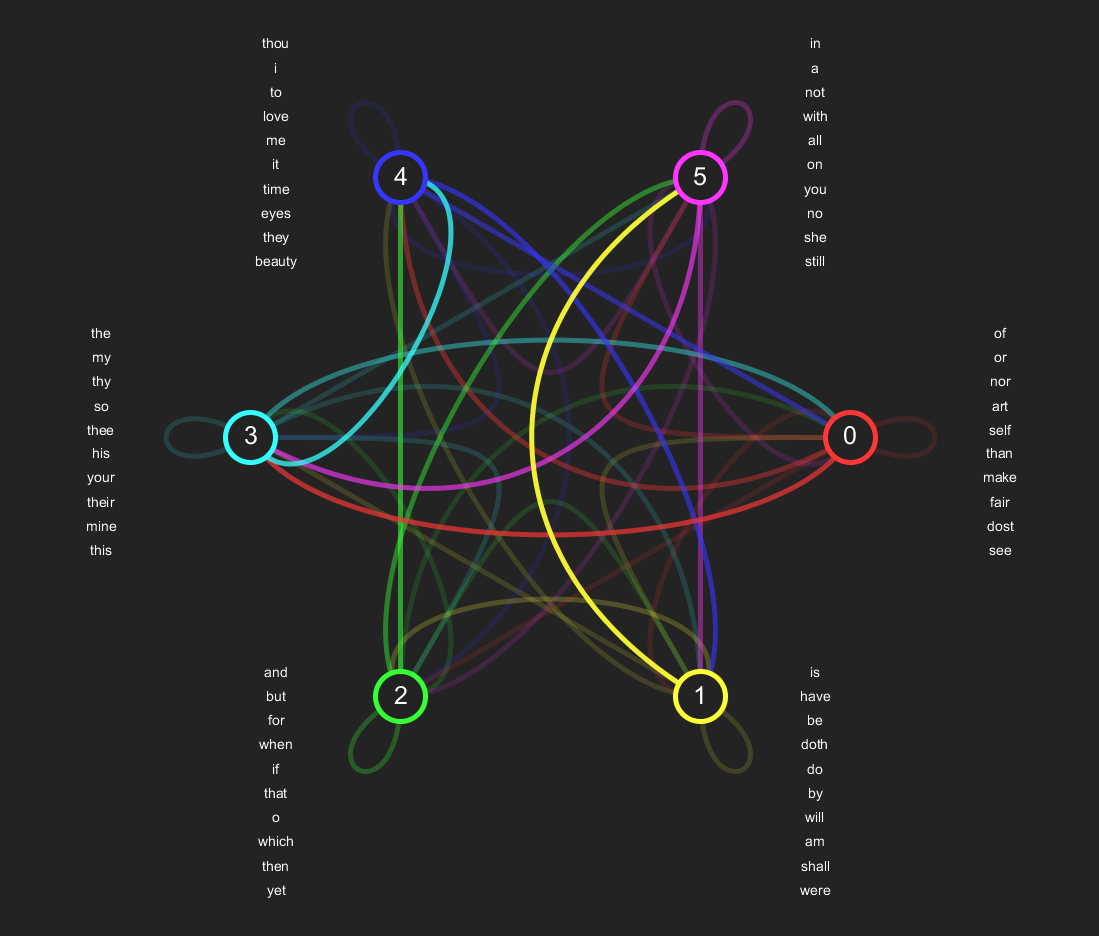
\includegraphics[scale=.4]{states.png}
    \end{center}

    \pagebreak

    \begin{itemize}
    \item \textbf{State Analysis:}
        We notice that state 1 has a high collection of verbs. This continues
        as well: checking the top 20 words for state 1 yields ``are, may, was,
        should, say, did, must, know, might, away'', which is further composed
        mostly of verbs. \\

        State 1 has the highest probability of transitioning to state 5, which
        contains mainly prepositions and some nouns (which correctly follow
        from verbs). \\

        State 5 has the highest probability of transitioning to state 3, which
        has several possesive nouns. Inspecting the top 20 words of state 3
        yields more possesive nouns such as ``her, thine, our'', and also
        some adjectives. \\

        State 3 then has the highest probability of transitioning to state 4,
        which contains even more nouns, as the sentence at this point, if
        began at state 3 (a likely verb), should reach the noun the verb is
        modifying. \\

        State 4 then has similar probabilities of transitioning to states 1
        and 0, which allow for more compound phrases. Since the HMM mainly
        trained on single lines of the sonnets, taking more than 9 transitions
        almost guarantees a grammerless phrase. The average number of words
        per line in all of the sonnets is just over 8, thus the HMM has
        difficulty outputing coherent long phrases.
    \end{itemize}

\end{itemize}



%%%%%%%%%%%%%%%%%%%%%%%%%%%%%%%%%%%%%%%%%%%%%%%%%%%%%%%%%%%%%%%%%%%%%%%%%%%%%%%%%%%%%%%%

\section{Poetry Generation}
\medskip
\begin{itemize}
    % In your report, describe your algorithm for generating the 14 line sonnet. Include at least one sonnet generated from your unsupervized trained HMM in your final report as an example. You should comment on the quality of geneating poems in this naive manner. How is the accurate is rhyme, rythym, and syllable count to what a sonnet should be? Do your poems make any sense? Does it retain Shakespeare’s original voice? How does training with different number of hidden states effect the poems generated (in a qualita- tive manner)? For the good qualities that you describe, also discuss how you think the HMM was able to capture these qualities.

    %%%%%%%%%%%%%%%%%%%%%%
    \item \boldline{Algorithm}

    \begin{itemize}
    \item \textbf{Two example non-naive sonnets:}
    \begin{verbatim}
        1  She have not eyes bright be that tiger's moan
        2  Every must change touches thou moan bed
        3  But the gold shook all so let and upon
        4  Everywhere to although stain full unbred
        5  To and i'll so shows care more releasing
        6  Be it thee thou fore when your which rehearse
        7  They the rage these life of mine possessing
        8  Painting therefore thine night a for inhearse
        9  His thy spurring prove so from are compiled
        10 In leisure in and seeing receives cry
        11 To touches strangle thy the to me filed
        12 Him my that saith they have my jollity
        13     Remain lawful hast I say 'will' annoy
        14     A under is his name strong thinks fled joy

        1  If breath to were book you due look rotten
        2  Line his in or you steeled my thee shown
        3  If wilful-slow grace me when forgotten
        4  Of every pen loving summer own
        5  Me going deserve with filching not guard
        6  Is dear of love in paying live it leaves
        7  Blame ever worst o what gazing since ward
        8  Your for candles distraction there be sheaves
        9  Excel heart others small invention light
        10 The with write way thy so health ignorance
        11 Then which thus do beweep need'st them aright
        12 And an far day back my in count advance
        13     All and face lo an sweets sight over-plus
        14     My respect triumph it uncertain thus
    \end{verbatim}

    \item \textbf{Algorithm:}


    \end{itemize}

    %%%%%%%%%%%%%%%%%%%%%%
    \item \boldline{Quality of generated poems}
    \begin{itemize}
        \item \textbf{Rhyme and the rhyming dictionary:} We forced rhyming by creating a rhyming dictionary of all of Shakespeare's ending words. We iterated through the sonnets, creating pairs of rhyming words using the known rhyme scheme ``ababcdcdefefgg'', then used a clumping algorithm to create super-pairs. For example, $(head, bed)$ and $(head, dead)$ would combine to $(head,bed,dead)$, then search again for additional matches. So, when building a line, we would pick a random rhyming word, build the line `backwards', then pick another rhyming word from the rhyming set (sometimes the same word if the size of the set was one), then repeat. Then, once we had 7 rhyming lines, we simply organized them into the ``ababcdcdefefgg'' rhyme scheme.
        \item \textbf{Rhythmn:} 
        \item \textbf{Syllables:} In order to have 10 syllables, per line, we ran a script to gather data on the average number of words per line in Shakespeare's sonnet. The distribution was approximately ([5 words] * 2 , [6 words] * 15 , [7 words] * 41 , [8 words] * 70 , [9 words] * 63 , [10 words] * 25). We used this distribution data to pick a random number of words, generated that many words (minus one, since we picked the ending word to force rhyming), then would continously generate new lines until we had a line that was 10 syllables using our counting algorithm.
        To count the number of syllables in a line, we mostly used the NLTK. However, there were some words used by Shakespeare that were not included in the NLTK. So, we supplemented this process with a less-accurate but still quite useful syllable-counting algorithm that would give its best guess wherever NTLK failed.
        \item \textbf{Grammar:} The grammar was perhaps the most difficult part of the poems. On occasion, we would get two words in a row, such as ``I I'' or ``the the''. More commonly, we would see two parts-of-sentence that did not make sense together, such as ``a the'', ``an a'', or ``thee thou''.
        \item \textbf{Punctuation:} Since we stripped all punctuation during pre-processing, there was minimal punctuation afterwards. Most notably, we would occasionally see the word `Will', with the apostrophes. We could have easily added ending punctuation, since Shakespeare has a fairly consistent style of $,,,:,,,:,,,:,.$ as line endings. However, we chose not to, for aesthetic reasons.
    \end{itemize}

\end{itemize}

%%%%%%%%%%%%%%%%%%%%%%%%%%%%%%%%%%%%%%%%%%%%%%%%%%%%%%%%%%%%%%%%%%%%%%%%%%%%%%%%%%%%%%%%

\section{Additional Goals}
\medskip
\begin{itemize}
    % Talk about the extra improvements you made to your poem generation algorithm. What was the prob- lems you were trying to fix? How did you go about attempting to fix it? Why did you think that what you tried would work? Did your method succeed in making the sonnet more like a sonnet? If not, why do you think what you tried didn’t work? What tradeoffs do you see in quality and creativity when you make these changes?

    %%%%%%%%%%%%%%%%%%%%%%
    \item \boldline{Improving poem quality}

    \begin{itemize}
    \item \textbf{Grammar:}
    \item \textbf{Rhyme scheme:}
    \item \textbf{Syllables:}
    \item \textbf{Punctuation:}
    \end{itemize}

\end{itemize}

%%%%%%%%%%%%%%%%%%%%%%%%%%%%%%%%%%%%%%%%%%%%%%%%%%%%%%%%%%%%%%%%%%%%%%%%%%%%%%%%%%%%%%%%

\end{document}